\documentclass[12pt]{extarticle}
\def\activityid{F04-M-v3}\usepackage[letterpaper,margin=.65in,top=.60in,bottom=.65in]{geometry}
\usepackage{fix-cm}
\usepackage[T1]{fontenc}\usepackage[default]{sourcesanspro}
\usepackage{microtype,tikz,array,tabularx,fancyhdr,amsmath,amssymb}
\usepackage[hidelinks]{hyperref}\usetikzlibrary{calc,arrows.meta}
\setlength{\parindent}{0pt}\setlength{\parskip}{7pt}\setlength{\headheight}{0pt}\setlength{\footskip}{26pt}
\setlength{\emergencystretch}{2em}\pagestyle{fancy}\fancyhf{}\renewcommand{\headrulewidth}{0pt}\renewcommand{\footrulewidth}{.4pt}
\fancyfoot[L]{\scriptsize Bellingham Math Circle / Week 4 / \activityid}\fancyfoot[R]{\scriptsize \thepage}
\definecolor{ink}{gray}{.12}\definecolor{soft}{gray}{.95}\color{ink}
\newcommand{\PageTitle}[2]{{\fontsize{10}{12}\selectfont\bfseries WEEK 4\quad ROUND AND ROUND\hfill #1\par}\vspace{3pt}{\fontsize{26}{29}\selectfont\bfseries #2\par}\vspace{2pt}}
\newcommand{\NameLine}{{\small Name: \rule{2.65in}{.4pt}\hfill Date: \rule{1.35in}{.4pt}\par}\vspace{4pt}}
\newcommand{\Task}[2]{\par\vspace{3pt}{\large\bfseries #1}\par #2\par}
\newcommand{\Subhead}[1]{\par\vspace{3pt}{\large\bfseries #1}\par}
\newcommand{\RuleBox}[1]{\par\begingroup\setlength{\fboxsep}{8pt}\colorbox{soft}{\parbox{\dimexpr\linewidth-16pt\relax}{#1}}\endgroup\par}
\newcommand{\WriteBox}[2]{\par\textbf{#1}\par\vspace{2pt}\begin{tikzpicture}\draw[black!40,line width=.5pt] (0,0) rectangle (\dimexpr\linewidth-.5pt\relax,#2);\end{tikzpicture}\par}
\newcommand{\StudentFooter}{\vfill{\small Try it with objects. Explain by pointing, talking, or drawing.}\par}
\newcommand{\LampRing}[3]{\begin{tikzpicture}[x=1in,y=1in]
\foreach \i in {1,...,#1}{\coordinate (v\i) at ({90-360*(\i-1)/#1}:#2);}
\foreach \i in {1,...,#1}{\pgfmathtruncatemacro{\j}{mod(\i,#1)+1}\draw[thick] (v\i)--node[midway,fill=white,inner sep=2pt,font=\small]{\i\j}(v\j);}
\foreach \i in {1,...,#1}{\node[circle,draw,fill=white,minimum size=.52in,inner sep=0pt,font=\bfseries] at(v\i){\i};}
\foreach \i in {#3}{\node[circle,draw,fill=ink,text=white,minimum size=.52in,inner sep=0pt,font=\bfseries] at(v\i){\i};}
\end{tikzpicture}}
\newcommand{\Lights}[1]{\begin{tikzpicture}[x=.55in,y=.55in,baseline=-.10in]\foreach \v [count=\i] in {#1}{\ifnum\v=1\fill (\i,0) circle(.16in);\else\draw (\i,0) circle(.16in);\fi}\end{tikzpicture}}
\newcommand{\ClockRing}[2]{\begin{tikzpicture}[x=1in,y=1in]\draw[black!30] (0,0) circle(#2);\pgfmathtruncatemacro{\n}{#1-1}\foreach\i in {0,...,\n}{\node[circle,draw,fill=white,minimum size=.35in,inner sep=0pt] at({90-360*\i/#1}:#2){\i};}\draw[-{Stealth},thick] (-.35,.15) arc(155:25:.38);\node[font=\small] at(0,-.18){clockwise};\end{tikzpicture}}
\newcommand{\Key}[2]{\begin{center}\renewcommand{\arraystretch}{1.55}\begin{tabular}{c|*{#1}{c}}in&#2\end{tabular}\end{center}}


% v3 student pages use one running header and numbered tasks only.
\newcommand{\StudentHeader}[1]{{\fontsize{10}{12}\selectfont\bfseries Week 4 / Ring shifts / #1\par}\vspace{10pt}}
\newcommand{\Problem}[2]{\par\vspace{4pt}\textbf{Problem #1:} #2\par}
\newcommand{\Space}[1]{\begin{tikzpicture}\draw[black!35] (0,0) rectangle (\dimexpr\linewidth-.5pt\relax,#1);\end{tikzpicture}\par}
\newcommand{\Record}[2]{#1\par\Space{#2}}

\begin{document}
\StudentHeader{Grades 2--3}

\Problem{1}{Use a counter on this ring. A turn moves a fixed number of places clockwise; after J comes A. Try a two-place turn from A, then from I. Record the two landings. Count places moved, not the starting place.}
\begin{center}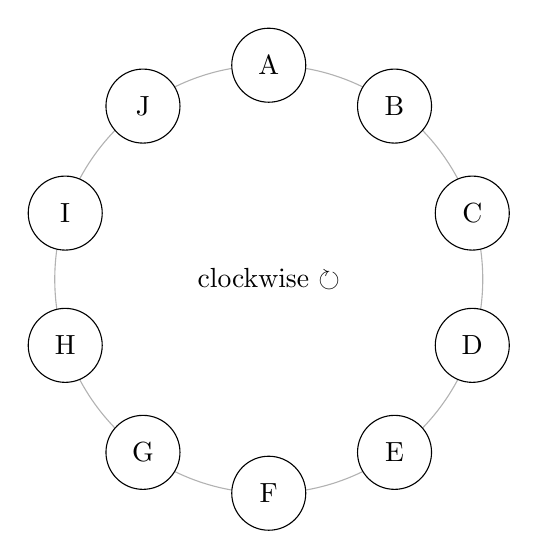
\begin{tikzpicture}[x=1in,y=1in]\draw[black!30](0,0)circle(1.07);\foreach\i/\l in {0/A,1/B,2/C,3/D,4/E,5/F,6/G,7/H,8/I,9/J}{\node[circle,draw,fill=white,minimum size=.37in]at({90-36*\i}:1.07){\l};}\node at(0,0){clockwise $\circlearrowright$};\end{tikzpicture}\end{center}
\Problem{2}{A secret turn takes A to D. Find its step size. Use that same turn from B, I, and J. Record the three outputs.}
\Space{.8in}
\Problem{3}{Encode BAG by shifting each letter with the secret turn. Decode GDG by undoing that turn. Check both messages by reversing your moves.}
\Space{.8in}
\Problem{4}{Someone says B becomes F with that same key. Test the claim on the ring. Record what B actually becomes.}
\Space{.55in}

\newpage
\StudentHeader{Grades 2--3}

\Problem{5}{Start at A. Take two clockwise places every turn. Record each landing until A first returns. Repeat from B. Do not record letters you pass over.}
\begin{center}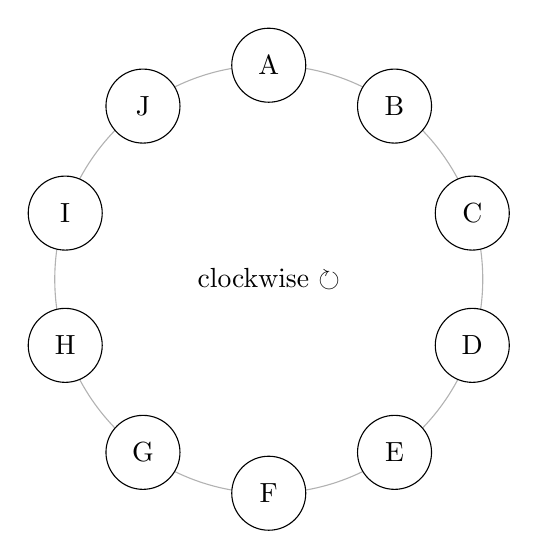
\begin{tikzpicture}[x=1in,y=1in]\draw[black!30](0,0)circle(1.07);\foreach\i/\l in {0/A,1/B,2/C,3/D,4/E,5/F,6/G,7/H,8/I,9/J}{\node[circle,draw,fill=white,minimum size=.37in]at({90-36*\i}:1.07){\l};}\node at(0,0){clockwise $\circlearrowright$};\end{tikzpicture}\end{center}
\Record{Start A: A $\to$}{.55in}\Record{Start B: B $\to$}{.55in}
\Problem{6}{Try the two-place rule from C, then from D. Compare with your first two routes. Circle which route each new start joins.}
\begin{center}\renewcommand{\arraystretch}{1.7}\begin{tabular}{c|cc}Start&Joins A's route&Joins B's route\\\hline C&yes / no&yes / no\\D&yes / no&yes / no\end{tabular}\end{center}
\Problem{7}{Mark the A-route letters with a dot and the B-route letters with a small cross on the ring. Follow one more turn from each letter and compare its marking with the next landing.}

\newpage
\StudentHeader{Grades 2--3}

\Problem{8}{Use the page-2 ring. From A, take three places per turn and record the complete route until A first returns. Compare its visited letters with the two-place routes.}
\Space{1in}
\Problem{9}{Test five-place turns from A, then from B. Draw the two routes. Compare their lengths with the two-place and three-place routes.}
\Space{1in}
\Problem{10}{A two-place route skips letters. Test whether you can still undo a two-place move from A, B, I, and J. Find one clockwise step size that brings every test back. Record each out-and-back trip.}
\Space{1.25in}
\Problem{11}{Choose a new step size from 1 to 9. Predict whether it visits all ten letters from A. Test and record its route.}
\Space{1.25in}

\end{document}
